
\section{Pré-traitements}
Avant de réaliser l'emploi du temps, nous procédons à des vérifications sur les données d'entrées afin de détecter toutes les incohérences. Ainsi, nous éliminons au préalable une partie des traitements qui n'aboutiront pas.

\subsection{Le nombre de professeurs}
La première vérification concerne le nombre de professeurs en entrée. Nous vérifions qu'il y a assez de professeurs pour dispenser les cours de chaque classe.
Ainsi pour un cours donné, l'algorithme somme les disponibilités des professeurs puis compare le résultat au nombre de classe, en tenant compte du fait que pour des cours de 4h, le nombre de disponibilités nécessaire est doublé.\\

Soit $n$ le nombre de professeurs pouvant donner un cours $c$ et $m$ le nombre de classes devant suivre ce cours.
Pour un cours de 2 heures, nous avons:
\begin{center}
$\sum_{i=0}^n dispo_{prof_i} > m$
\end{center}

Pour un cours de 4 heures, nous avons: 
\begin{center}
$\frac{\sum_{i=0}^n dispo_{prof_i}}{2} > m$
\end{center}

Pour un cours dispensé sur 4h, le nombre de disponibilités nécessaire est doublé. Pour simplifier nos calculs, nous divisons par 2 le nombre de disponibilités trouvées pour un professeur pour le comparer aux disponibilités nécessaires pour dispenser le cours.

L'opération est répétée pour l'ensemble des cours. 

\newpage

\begin{algorithm}
\caption{Pré-traitement du nombre de professeurs}
\begin{algorithmic}
\FORALL{$Cours$}
\STATE $idCours \leftarrow$ identifiant de $Cours$
\STATE $idPromo \leftarrow$ identifiant de la promotion recevant $Cours$
\STATE $nbClasses \leftarrow$ nombre de classe de la promotion $idPromo$
\FORALL{$Profs$}
\IF {$Profs$ donne le cours $idCours$}
\FORALL {$CreneauxProf$}
\IF {$Profs$ est disponible}
\STATE $nbCreneaux \leftarrow nbCreneaux + 1$
\ENDIF
\ENDFOR
\ENDIF
\ENDFOR
\IF {$Cours$ est sur 4h}
\STATE $nbCreneaux \leftarrow nbCreneaux / 2$
\ENDIF
\IF{$nbClasses > nbCreneaux$}
\STATE display (Erreur sur le nombre de professeurs pour la promotion $idPromo$)
\STATE EXIT FAILURE
\ENDIF
\ENDFOR
\STATE display (Nombre de professeurs ok)
\end{algorithmic}
\end{algorithm}

\subsection{Le nombre de cours total sur le semestre}
La seconde vérification porte sur le nombre d'heures de cours à dispenser à une classe. Ce nombre ne doit pas excéder la totalité des heures du semestre. Le programme somme l'ensemble des cours que possède une classe et le compare au nombre d'heures total du semestre.

\begin{center}
$\sum_{i=0}^n nbHeures_{cours_i} \leq s*c*h$
\end{center}

Avec :
\begin{itemize}
\item $n$ le nombre de cours d'une classe
\item $s$ le nombre de semaines du semestre
\item $c$ le nombre de créneaux sur une semaine
\item $h$ le nombre d'heures d'un créneau
\end{itemize}

\newpage

\begin{algorithm}
\caption{Pré-traitement du nombre d'heures sur le semestre}
\begin{algorithmic}
\FORALL{$Classes$}
\STATE $listCours \leftarrow$ ensemble des cours que suit une classe
\FORALL {$cours$ in $listCours$}
\STATE $nbHours \leftarrow nbHours $ + nombre d'heures du cours $cours$
\ENDFOR
\IF {$nbHours$ > (nombre de semaines du semestre * nombre de créneaux par semaine * nombre d'heures par créneau)}
\STATE display(Erreur, trop d'heures pour la classe $Classes$)
\STATE EXIT FAILURE
\ENDIF
\ENDFOR
\STATE display(Nombre d'heures de cours ok)
\end{algorithmic}
\end{algorithm}

Une fois ces pré-traitements réalisés, nous pouvons commencer la conception de l'emploi du temps.

\newpage
\section{Réalisation de l'emploi du temps}
Il est difficile de trouver une solution exacte pour un problème d'ordonnancement, donc pour faciliter la génération de l'emploi du temps, nous avons mis en place une fonction de répartition aléatoire des cours dans la semaine. Cette fonction est rappelée un certain nombre de fois (nombre d'itérations à définir), mais le programme s'arrête si une solution est trouvée avant la dernière itération.\\

Afin de clarifier l'explication, nous rappelons que le programme de l'année est un ensemble de matières (Algèbre, Analyse, Electricité, etc.), et que chaque matière est un ensemble de cours (Algèbre : 14 cours de 2h, Analyse 12 cours de 2h, etc.), répartis sur les créneaux de la semaine. De plus, chaque promotion (B1, B2, B3, etc.) est constituée d'un certain nombre de classes (B1A, B2C, M1B, etc.).
Enfin, un créneau correspond à 2h dans la semaine (Lundi 8h30-10h30, Mercredi 14h-16h, etc.), un cours de 2h se place donc sur un créneau, et un cours de 4h sur 2 créneaux.\\

Afin d'optimiser la répartition des cours dans la semaine, nous répartissons au préalable les matières du programme, et les enseignants correspondant sur le semestre, et ce pour chaque promotion. Ainsi, chaque classe d'une même promotion suivra les mêmes cours chaque semaine, ce qui garantit l'homogénéité de l'emploi du temps.\\

Pour ce faire, nous déterminons la semaine à laquelle doit se dérouler le premier cours de chaque matière, ainsi que le nombre de semaines nécessaires. Nous pouvons alors répartir les cours sur chaque semaine à l'aide de la fonction de répartition aléatoire. Cette fonction sera rappelée jusqu'à trouver une solution dans laquelle tous les cours ont été placés correctement. En cas d'échec (aucune solution parfaite), le programme donnera la solution dans laquelle un minimum de cours n'ont pas été placés correctement. Ces cours pourront toutefois être placés manuellement par la suite.\\

\newpage

\begin{algorithm}
\caption{Principe général de conception des emplois du temps}
\begin{algorithmic}
\STATE $meilleurEDT \leftarrow \infty$
\REPEAT
\FORALL{$Promo$}
\STATE $idMatieres \leftarrow$ liste contenant les id des matières que doivent suivrex $Promo$
\STATE $programmeSemestre \leftarrow $ liste contenant la répartition des $idMatieres$ sur le semestre
\STATE $planningOk \leftarrow$ booléen indiquant si la génération de l'emploi du temps a rencontré des erreurs
\ENDFOR
\IF {$planningOk$}
\IF {$nbCoursNonPlaces < meilleurEDT$}
\STATE $meilleurEDT \leftarrow nbCoursNonPlaces$
\STATE Ecriture des emplois du temps dans les fichiers
\ENDIF
\ENDIF
\UNTIL {meilleurEDT > 0 \AND cmpt < nombreIteration}
\end{algorithmic}
\end{algorithm}

\subsection{Répartition du programme sur le semestre}

Afin d'optimiser la répartition des cours sur chaque semaine, nous commençons par répartir les matières sur les semaines du semestre. Pour chaque matière, nous allons donc indiquer la semaine dans laquelle doit commencer le premier cours, ainsi que le nombre de semaines durant lequel elle va être enseignée.\\

La répartition se déroule en deux étapes : 
\begin{itemize}
\item Le tri des matières 
\item Le placement des matières sur le semestre\\
\end{itemize}

L'objectif est de répartir les cours sur le semestre de manière homogène. Il faut donc réussir à placer le maximum de matières les unes à la suite des autres. Pour ce faire, nous trions les matières de la plus longue à la plus courte (en nombre de semaines), puis nous les plaçons les unes après les autres dans le semestre, en faisant en sorte de les placer à la suite d'une autre matière dès que possible.

\newpage

\begin{figure}[! ht ]
    \centering
    \begin{minipage}[t]{14 cm}
        \centering
            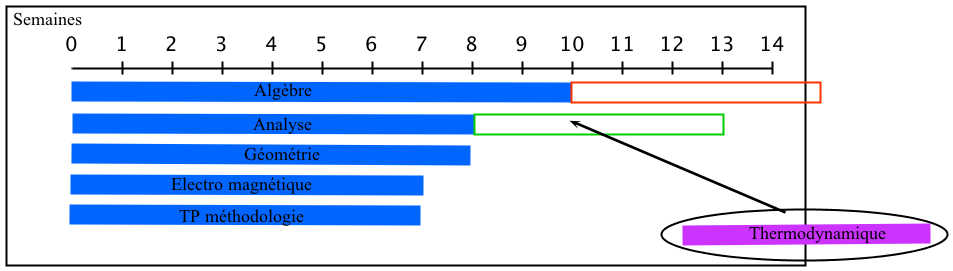
\includegraphics [width=160mm, height=60mm]{RepartitionSemestre2.png}
        \caption {Ajout d'un cours à la suite d'un autre sur le semestre}
    \end{minipage}
\end{figure}

Un cours de 4 heures impose plus de contraintes. En effet, il s'agit d'un cours où le professeur et la classe doivent avoir en commun deux créneaux libres consécutifs dans la même demi-journée. C'est pourquoi un cours de 4 heures doit être planifié sur le semestre avant un cours de 2 heures.\\

Pour ce faire, les matières sont séparées en deux listes : une pour les cours de 4 heures et une autre pour les cours de 2 heures, et nous effectuons les répartitions sur le semestre comme expliqué précédemment.\\

\begin{figure}[! ht ]
    \centering
    \begin{minipage}[t]{14 cm}
        \centering
            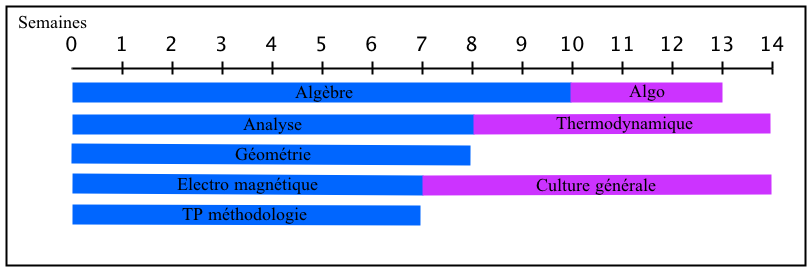
\includegraphics [width=160mm, height=60mm]{RepartitionSemestre.png}
        \caption {Modélisation du planning du semestre}
    \end{minipage}
\end{figure}


Pour chaque matière, nous avons besoin des informations suivantes :
\begin{itemize}
\item L'identifiant de la matière
\item Le numéro de la semaine dans laquelle sera donné le premier cours
\item Le nombre de semaines nécessaires pour enseigner l'ensemble de la matière
\item La matière qui la suit, s'il y en a une
\end{itemize}

\begin{algorithm}
\caption{Algorithme principal de la répartition des matières sur le semestre}
\begin{algorithmic}
\REQUIRE liste $idMatieres$, liste $programmeSemestre$
\FORALL {$idMatieres$}
\IF {$idMatieres$ est un cours sur 2h}
\STATE $idMatieres2 \leftarrow$ pushback $idMatieres$
\ELSE
\STATE $idMatieres4 \leftarrow$ pushback $idMatieres$
\ENDIF
\ENDFOR
\STATE Tri de $idMatieres2$ par nombre de semaines de matière décroissant
\STATE Tri de $idMatieres4$ par nombre de semaines de matière décroissant
\STATE $idMatieres$ est vidé
\FORALL {$idMatieres4$}
\STATE $idMatieres \leftarrow$ pushback $idMatieres4$
\ENDFOR
\FORALL {$idMatieres2$}
\STATE $idMatieres \leftarrow$ pushback $idMatieres2$
\ENDFOR
\RETURN $programmeSemestre \leftarrow$ repartitionDesCours($idMatieres$)
\end{algorithmic}
\end{algorithm}

\begin{algorithm}
\caption{repartitionDesMatieres($idMatieres$)}
\begin {algorithmic}
\REQUIRE liste $idMatieres$ triée par nombre de semaines d'une matière et par cours de 4h et 2h
\STATE initialisation de $programmeSemestre$
\FORALL {$idMatieres$}
\FORALL {$Matieres$ in $programmeSemestre$}
\IF {$Matieres$ a été placé}
\STATE checkNextCourse($idCourses, Matieres$)
\IF {$idMatieres$ a été programmé}
\STATE $coursPlace \leftarrow true$
\STATE BREAK
\ENDIF
\ENDIF
\ENDFOR
\IF {$coursPlace == false$}
\STATE $programmeSemester \leftarrow$ pushback $idMatieres$ en le programmant en début de semestre
\ENDIF
\ENDFOR
\RETURN $programmeSemestre$
\end{algorithmic}
\end{algorithm}


\newpage

\begin{algorithm}
\caption{checkNextCourse($idMatieres, Matieres$)}
\begin {algorithmic}
\IF {$Matieres$ a une autre matière après lui}
\STATE checkNextCourse($idMatieres, Matieres$ du $Matieres$ suivant)
\ELSIF {$semaineDebut_{coursProgrammes} + nbSemaine_{coursProgramme} + nbSemaine_{idMatieres} \leq nbSemaine_{semestre}$}
\STATE $programmeSemestre \leftarrow$ pushBack $idMatieres$ en le programmant après le cours $Matieres$
\ENDIF
\end{algorithmic}
\end{algorithm}

Après avoir réalisé cet emploi du temps, nous pouvons commencer à placer les cours sur les créneaux des classes concernées.

\subsection{Répartion des cours sur leurs créneaux}

A partir de l'emploi du temps du semestre, nous allons planifier les cours sur les créneaux des classes. A la fin de chaque semaine, les classes d'une même promotion doivent être au même point du programme. Ainsi, l'emploi du temps est réalisé en parallèle pour chaque promotion semaine par semaine.

Pour chacune des semaines, nous allons récupérer la liste des cours à dispenser depuis l'emploi du temps semestriel. A partir des semaines de début et de fin de cours, nous en déduisons s'il doit être donné sur cette semaine.

Avec ce programme, nous allons pouvoir commencer à placer les cours sur les différents créneaux des classes. Cela va être fait en trois étapes : \\
\begin{itemize}
\item Si le cours a déjà été placé à la semaine précédente
\item La récupération de la liste des professeurs pouvant enseigner les cours de la semaine
\item Le placement des nouveaux cours du semestre\\
\end{itemize}

Dans le cas où un cours n'a pu être placé faute de créneaux disponibles, nous avons décidé de le mettre dans une liste contenant l'ensemble des cours non placés et de ne pas tenter de le replacer sur les semaines suivantes. Ainsi cette liste contiendra l'identifiant du cours, l'identifiant du professeur et les semaines où le cours n'a pu être placé.

\begin{algorithm}
\caption {Algorithme principal de la répartition des cours sur les créneaux des classes}
\begin{algorithmic}
\REQUIRE le programme du semaine $prog$
\FORALL{$semaine$ du semestre}
\STATE $progSemaine \leftarrow$ getProgrammeSemaine($prog, semaine$)
\STATE placementAncienCours($progSemaine, listeClasses, semaine$)
\IF {il y a des cours à placer encore dans la semaine}
\STATE $profSemaine \leftarrow$ getProfSemaine($progSemaine$)
\STATE placementNouveauCours($listeCalsses, progSemaine, profSemaine, semaine$)
\ENDIF
\IF {une erreur est survenu dans la réalisation du planning}
\RETURN 0
\ENDIF
\ENDFOR
\RETURN 1
\end{algorithmic}
\end{algorithm}

\begin{algorithm}
\caption{Méthode pour récupérer le programme d'une semaine}
\begin{algorithmic}
\REQUIRE le programme du semaine $prog$ et la semaine du semestre $semaine$
\FORALL {$cours$ du programme}
\IF {semaineDebut de $cours \leq semaine \AND $ semaine fin de $cours > semaine$}
\STATE $progSemaine \leftarrow$ pushback $cours$
\ENDIF
\ENDFOR
\RETURN $progSemaine$
\end{algorithmic}
\end{algorithm}

\subsubsection{Placement de cours déjà fixé la semaine précédente}

Après avoir récupéré le programme de la semaine, nous vérifions si l'un des cours a déjà été placé la semaine précédente. Si c'est le cas, nous allons vérifier que le professeur ayant donné le cours est toujours disponible sur le créneau et nous plaçons le cours.\\

Dans le cas où le cours a pu être redonner pour toutes les classes de la promotion, nous pouvons supprimer le cours dans le programme de la semaine. Sinon, soit il s'agit d'un nouveau cours, soit toutes les classes ne l'ont pas reçu. Ce dernier cas arrive lorsqu'un professeur n'est plus disponible ou quand le cours n'a pu être placé pour toutes les classes de la promotion.\\

Ceci va permettre à une classe d'avoir le même cours sur le même créneaux avec le même professeur semaine après semaine.

\begin{algorithm}
\caption{Méthode pour placer les cours précédemment planifier}
\begin{algorithmic}
\REQUIRE le programme de la semaine $prog$, la liste des classes $classes$, la semaine du semestre $semaine$
\STATE $nbCourseAjout \leftarrow 0$
\STATE $nouveauCours \leftarrow false$
\IF {La première semaine à déjà été planifié}
\FORALL {$cours$ du programme de la semaine}
\STATE coursDejaProgrammeAvant($cours, classes, nbCoursAjout, nouveauCours$)
\IF {$nbCoursAjout = $nombre $classes$}
\STATE $coursASupprimer \leftarrow$ pushback $cours$
\ELSE 
\STATE $nouveauCours \leftarrow faux$
\ENDIF
\STATE $nbCourseAjout \leftarrow 0$
\ENDFOR
\FORALL {$coursASupprimer$}
\STATE $progSemestre \leftarrow$ supprimer $progSemestre(coursASupprimer)$
\ENDFOR
\ENDIF
\end{algorithmic}
\end{algorithm}


\begin{algorithm}
\caption{Méthode pour savoir si un cours a déjà été programmé avant}
\begin{algorithmic}
\REQUIRE le cours de la semaine $cours$, la liste des classe $classes$ , la semaine du semestre $semaine$
\FORALL {$classes$}
\IF {$classes$ a reçu le cours la semaine $semaine -1$}
\STATE ajoutDuCours($classes, cours, semaine$)
\STATE $nbCoursAjoute \leftarrow nbCoursAjoute + 1$
\ENDIF
\ENDFOR
\IF {$nbCoursAjoute = $nombre de $classes$}
\STATE $nouveauCours \leftarrow faux$
\ELSE
\STATE $nouveauCours \leftarrow vrai$ 
\ENDIF
\end{algorithmic}
\end{algorithm}


\begin{algorithm}
\caption{Méthode pour ajouter le cours par rapport à la semaine d'avant}
\begin{algorithmic}
\REQUIRE la classe $classe$, la matière $cours$, la semaine du semestre $semaine$
\STATE $idProf \leftarrow $identifiant du professeur donnant $cours$ la $semaine - 1$
\STATE $creneau \leftarrow $créneau de $cours$ la $semaine - 1$
\IF {$cours$ est sur 4 heures}
\IF {$prof$ est disponible à $semaine, creneau \AND prof$ est disponible $semaine, creneau + 1 \AND classe$ est disponible à $semaine, creneau \AND classe$ est disponible $semaine, creneau +1$}
\STATE planification $cours$ avec $prof$ sur $semaine$ et $creneau$
\STATE planification $cours$ avec $prof$ sur $semaine$ et $creneau +1$
\ENDIF
\ELSE
\IF {$prof$ est disponible à $semaine, creneau \AND$ $prof$ est disponible $semaine, creneau + 1$}
\STATE planification $cours$ avec $prof$ sur $semaine$ et $creneau$
\ENDIF
\ENDIF
\end{algorithmic}
\end{algorithm}

\newpage

\subsubsection{Planification des nouveaux cours du semestre}

A partir du programme du semestre, nous récupérons l'ensemble des professeurs pouvant enseigner la liste des matières. Tous les professeurs ne se verront pas forcément attribuer un cours car plusieurs professeurs peuvent enseigner le même cours.\\

Pour tous les cours restant à planifier, nous allons à chaque fois trouver le couple promotion-professeur ayant le moins de créneaux en communs. En effet si nous plaçons des couples ayant plus de disponibilités avant un couple qui en a moins, il pourrait bloquer l'ensemble des disponibilités de ce dernier.\\

Ensuite, nous sélectionnons un créneaux aléatoirement parmi les choix possibles pour placer un cours. Nous réalisons un tirage aléatoire pour pouvoir essayer plusieurs combinaisons.\\

Dans le cas d'un cours de 4 heures, il se peut que nous n'ayons aucun créneau permettant de mettre les 4 heures à la suite. Dans ce cas nous mettons le cours dans la liste des cours n'ayant pu être planifié. 
Auquel cas, nous plaçons le cours de la classe sur le créneau en modifiant les disponibilités du professeurs. 

\begin{algorithm}
\caption {Méthode pour ajouter un nouveau cours}
\begin{algorithmic}
\REQUIRE $progSemaine, profSemaine, listClasses$
\STATE $nbCours \leftarrow $ nombre de cours dans $progSemaine * $ nombre de classe dans $listClasses$
\FOR {i := 0  \TO nbCours }
\STATE meilleurConnexion($progSemaine, profSemaine, listClasses, semaine$)
\IF {on trouve une connexion}
\STATE ajoutCours($progSemaine, profAAjouter, classesAAjouter, semaine$)
\ELSE
\RETURN 0
\ENDIF
\ENDFOR
\RETURN 1
\end{algorithmic}
\end{algorithm}

\newpage

\begin{algorithm}
\caption {Méthode pour trouver la plus meilleur connexion}
\begin{algorithmic}
\REQUIRE $progSemaine, profSemaine, listClasses, semaine$
\STATE $buf \leftarrow 23$
\FORALL {$profSemaine$}
\FORALL {$listClasses$}
\STATE $nbConnections \leftarrow $ nbCreneauCommun($profSemaine, listClasses, semaine$)
\IF {$nbConnections > 0 \AND nbConnections < buf$}
\STATE $buf \leftarrow nbConnections$
\STATE $profAAjouter \leftarrow profSemaine$
\STATE $promoAAjouter \leftarrow listClasses$
\ENDIF
\ENDFOR
\ENDFOR
\end{algorithmic}
\end{algorithm}

\begin{algorithm}
\caption {Méthode pour compter le nombre de connection}
\begin{algorithmic}
\REQUIRE $prof, classe, semaine, progSemaine$)
\FORALL {$cours$ donnés par $prof$}
\IF {$promo$ doit recevoir $cours$ sur $semaine$ \AND $cours$ n'a pas encore été placé pour $promo$ sur $semaine$}
\STATE $coursPossible \leftarrow vrai$
\STATE BREAK
\ELSE
\STATE $coursPossible \leftarrow faux$
\ENDIF
\ENDFOR
\IF {$coursPossible$}
\RETURN $nbConnection \leftarrow $ somme des disponibilité commune de $prof$ et $promo$
\ENDIF
\RETURN -1
\end{algorithmic}
\end{algorithm}

\newpage

\begin{algorithm}
\caption {Méthode pour ajouter un cours à une classe}
\begin{algorithmic}
\REQUIRE $progSemaine, profAAjouter, classesAAjouter, semaine$
\FORALL {$cours$ de $profAAjouter$}
\IF {$promo$ doit recevoir $cours$ sur $semaine$ \AND $cours$ n'a pas encore été placé pour $promo$ sur $semaine$}
\STATE creationCours($prof, promo, cours, semaine$)
\STATE BREAK
\ENDIF
\ENDFOR
\end{algorithmic}
\end{algorithm}

\newpage

\begin{algorithm}
\caption {Méthode pour créer le cours à la classe}
\begin{algorithmic}
\IF {$cours$ n'a pas été programmé à $semaine -1$ pour $classes$}
	\STATE ajout de $cours$ dans la liste des cours non planifié
\ELSIF {$cours$ est sur 4 heures}
	\FORALL {$creneau$}
		\IF {$classe$ est libre à $semaine, creneau$ \AND $classe$ est libre à $semaine, creneau + 1$ \AND $prof$ est libre à 			$semaine, creneau$  \AND $prof$ est libre à $semaine, creneau+1$ }
			\STATE $creneauxPossibles \leftarrow$ pushback $creneau$
		\ENDIF
	\ENDFOR
	\IF {$creneauxPossibles$ n'est pas vide}
		\STATE $creneau \leftarrow$ choix aléatoire dans $creneauxPossibles$
		\STATE mise en place du cours et des données ($cours, classe, prof, semaine, creneau$)
		\STATE mise en place du cours et des données ($cours, classe, prof, semaine, creneau +1$)
	\ENDIF
	\STATE ajout de $cours$ dans la liste des cours non planifié
\ELSE
	\FORALL {$creneau$}
		\IF {$classe$ est libre à $semaine, creneau$ \AND $prof$ est libre à $semaine, creneau$}
			\STATE $creneauxPossibles \leftarrow$ pushback $creneau$
		\ENDIF
	\STATE $creneau \leftarrow$ choix aléatoire dans $creneauxPossibles$
	\STATE mise en place du cours et des données ($cours, classe, prof, semaine, creneau$)
	\ENDFOR
\ENDIF
\end{algorithmic}
\end{algorithm}






\section{Déplacements des cours}

Une fois l'emploi du temps réalisé, nous avons la possibilité de déplacer des cours et/ou de placer manuellement les cours qui n'ont pu être placés lors de l'exécution du programme.

\subsection {Déplacement d'un cours existant}

Dans un premier temps, il faut choisir la classe pour laquelle nous souhaitons effectuer le changement. Ensuite nous sélectionnons le cours à déplacer, et la liste des créneaux communs au professeur et à la classe apparait. En sélectionnant le créneau dans lequel nous souhaitons déplacer le cours, le changement s'effectue directement en mettant à jour les données relatives à la plannification.

\subsection {Ajout d'un cours non placé}

La liste des cours non placés apparait. Il n'y a qu'à sélectionner le cours que nous voulons placer, et la liste des créneaux sur lequel il peut être placé apparait. Les instructions suivantes sont les mêmes que pour le déplacement d'un cours.